% Authored results moved from the application fiche; shared with its standalone.


The thermal bridges benchmark has been executed on the Gaya supercomputer at Unistra for the three mesh refinement levels (M1, M2, M3) using finite element approximations of order 1, 2, and 3. The results demonstrate both the accuracy of the numerical method through comparison with ISO 10211:2017 reference values, and the scalability of the implementation across multiple processors.
The results demonstrate both the accuracy of the numerical method through comparison with ISO 10211:2017 reference values, and the scalability of the implementation across multiple processors.

\subsubsection{Numerical solution}

\Cref{fig:spec:app-feelpp-discr-1:thermal_bridges:visualization} shows the computed temperature field and the mesh partitioning used for parallel computation. The temperature distribution exhibits the expected heat transfer patterns through the thermal bridge, with the coldest regions in blue and the warmest in red. The partitioning visualization (right panel) demonstrates the load balancing strategy employed by the domain decomposition method, where different colors represent different processor domains.

\begin{figure}[!ht]
  \centering
  \begin{subfigure}[c]{0.49\textwidth}
    \centering
    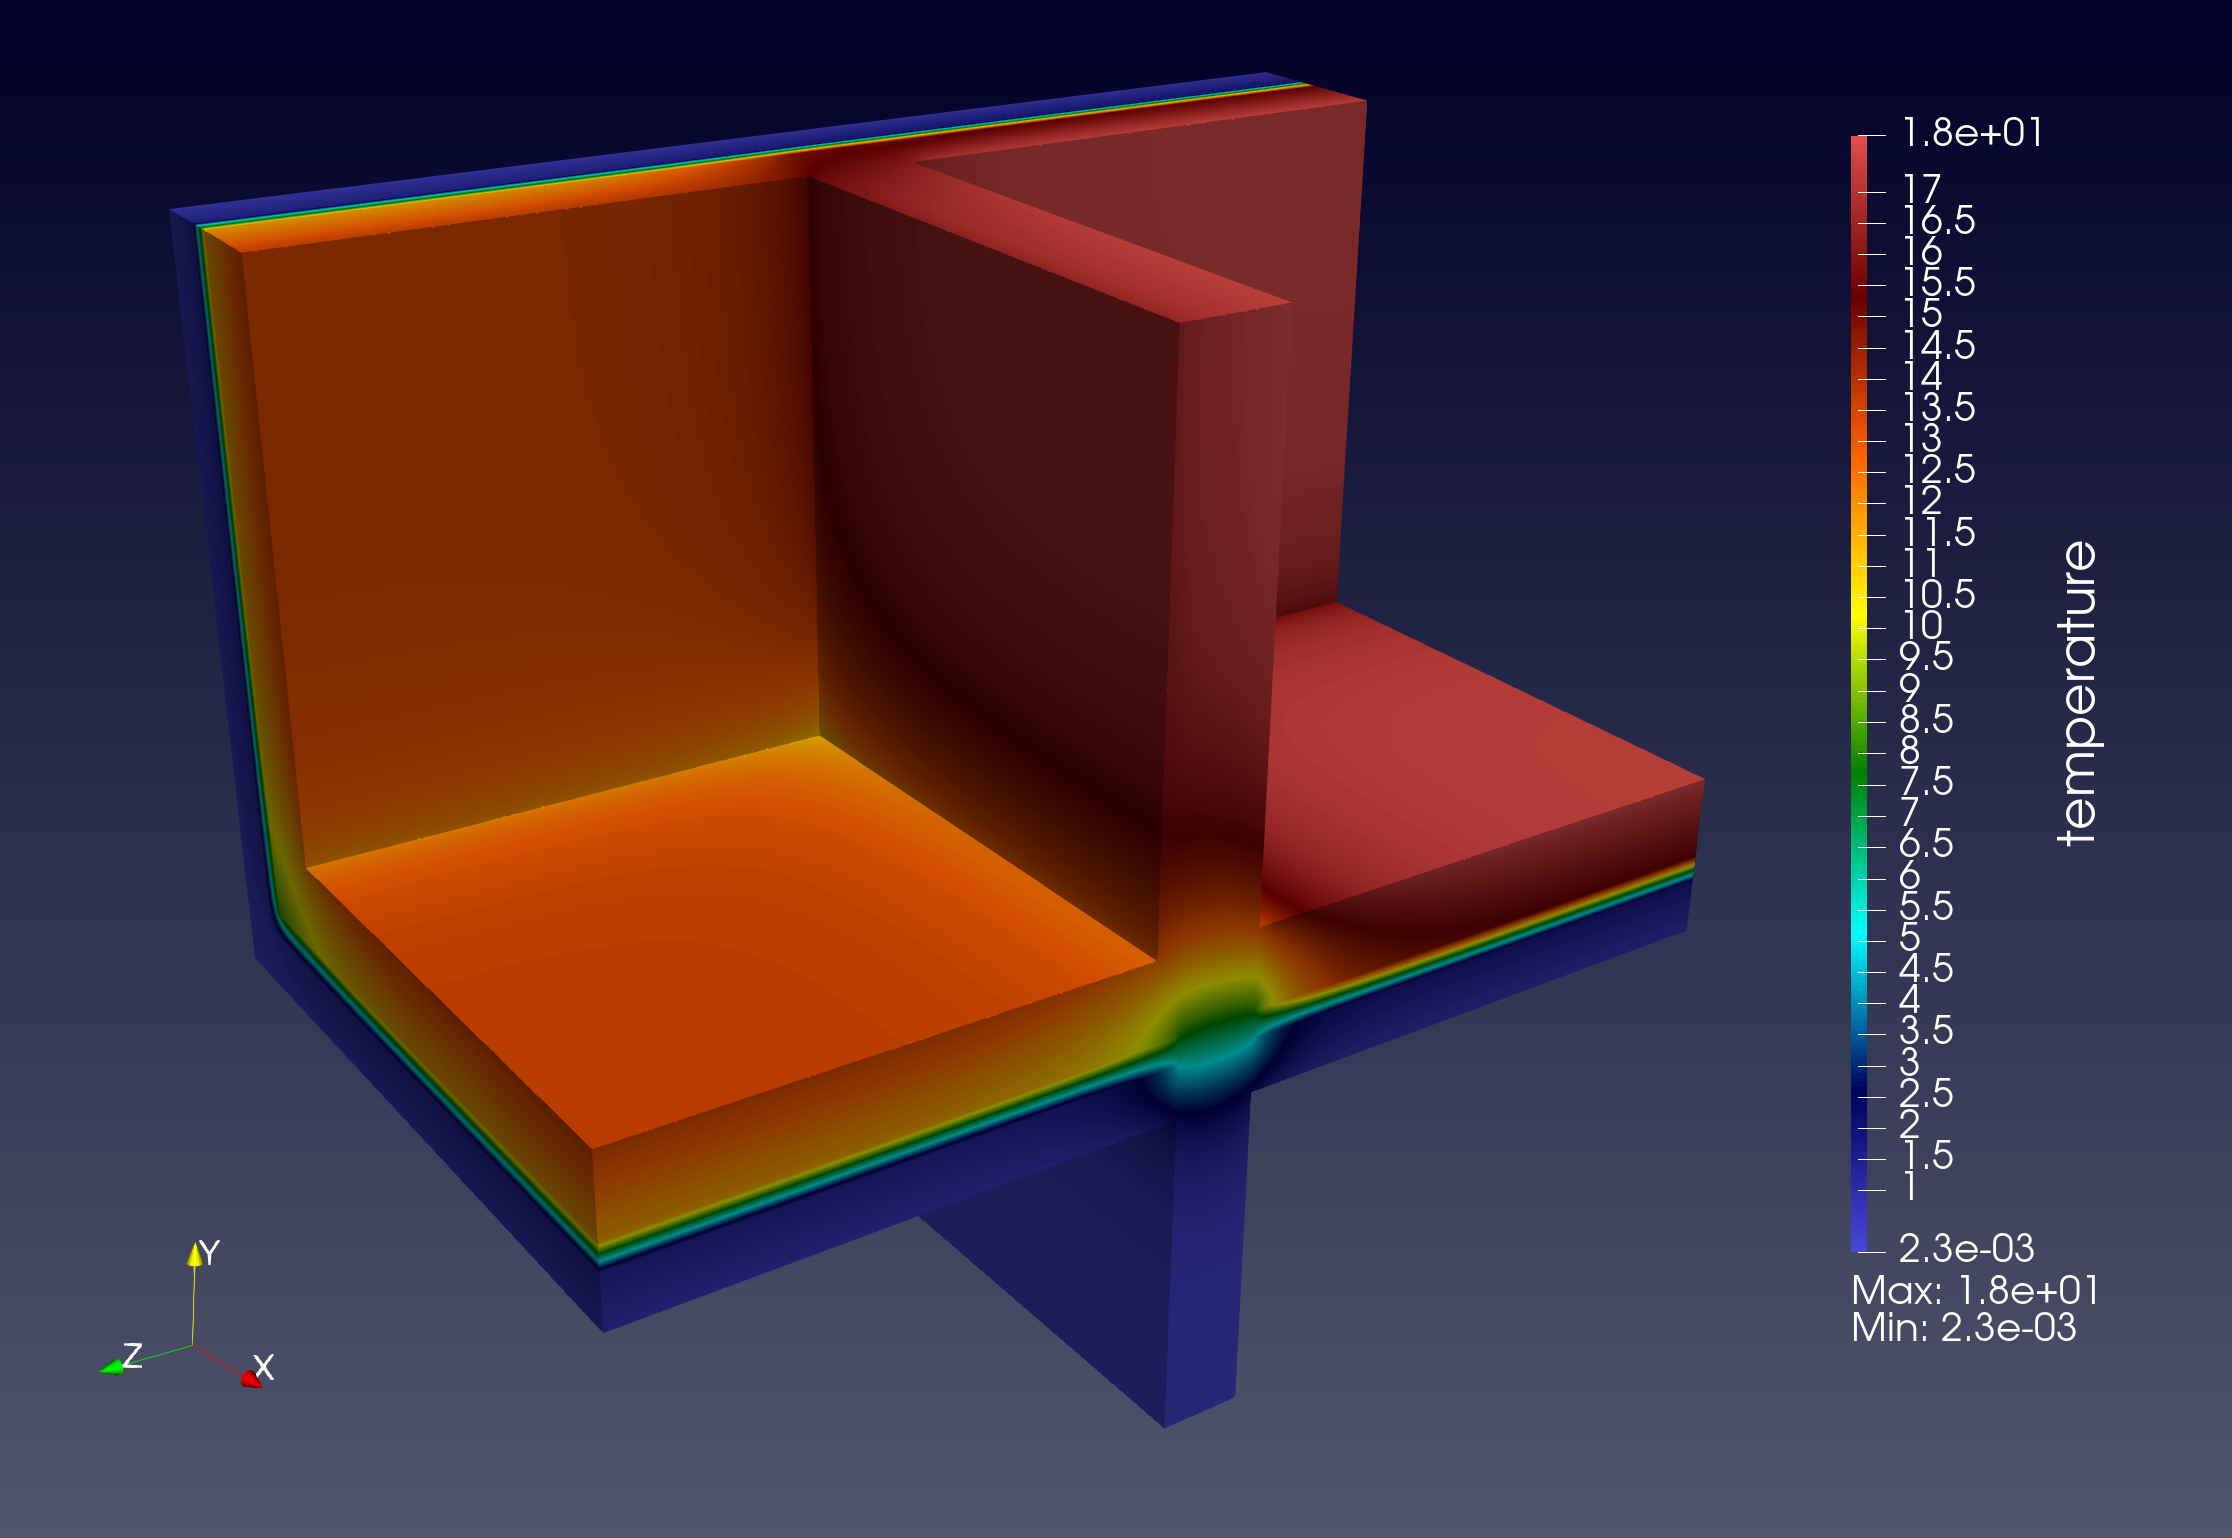
\includegraphics[width=\textwidth]{graphics/feelpp/feelpp-benchmark-thermalbridges-solution.png}
  \end{subfigure}
  \hfill
  \begin{subfigure}[c]{0.49\textwidth}
    \centering
    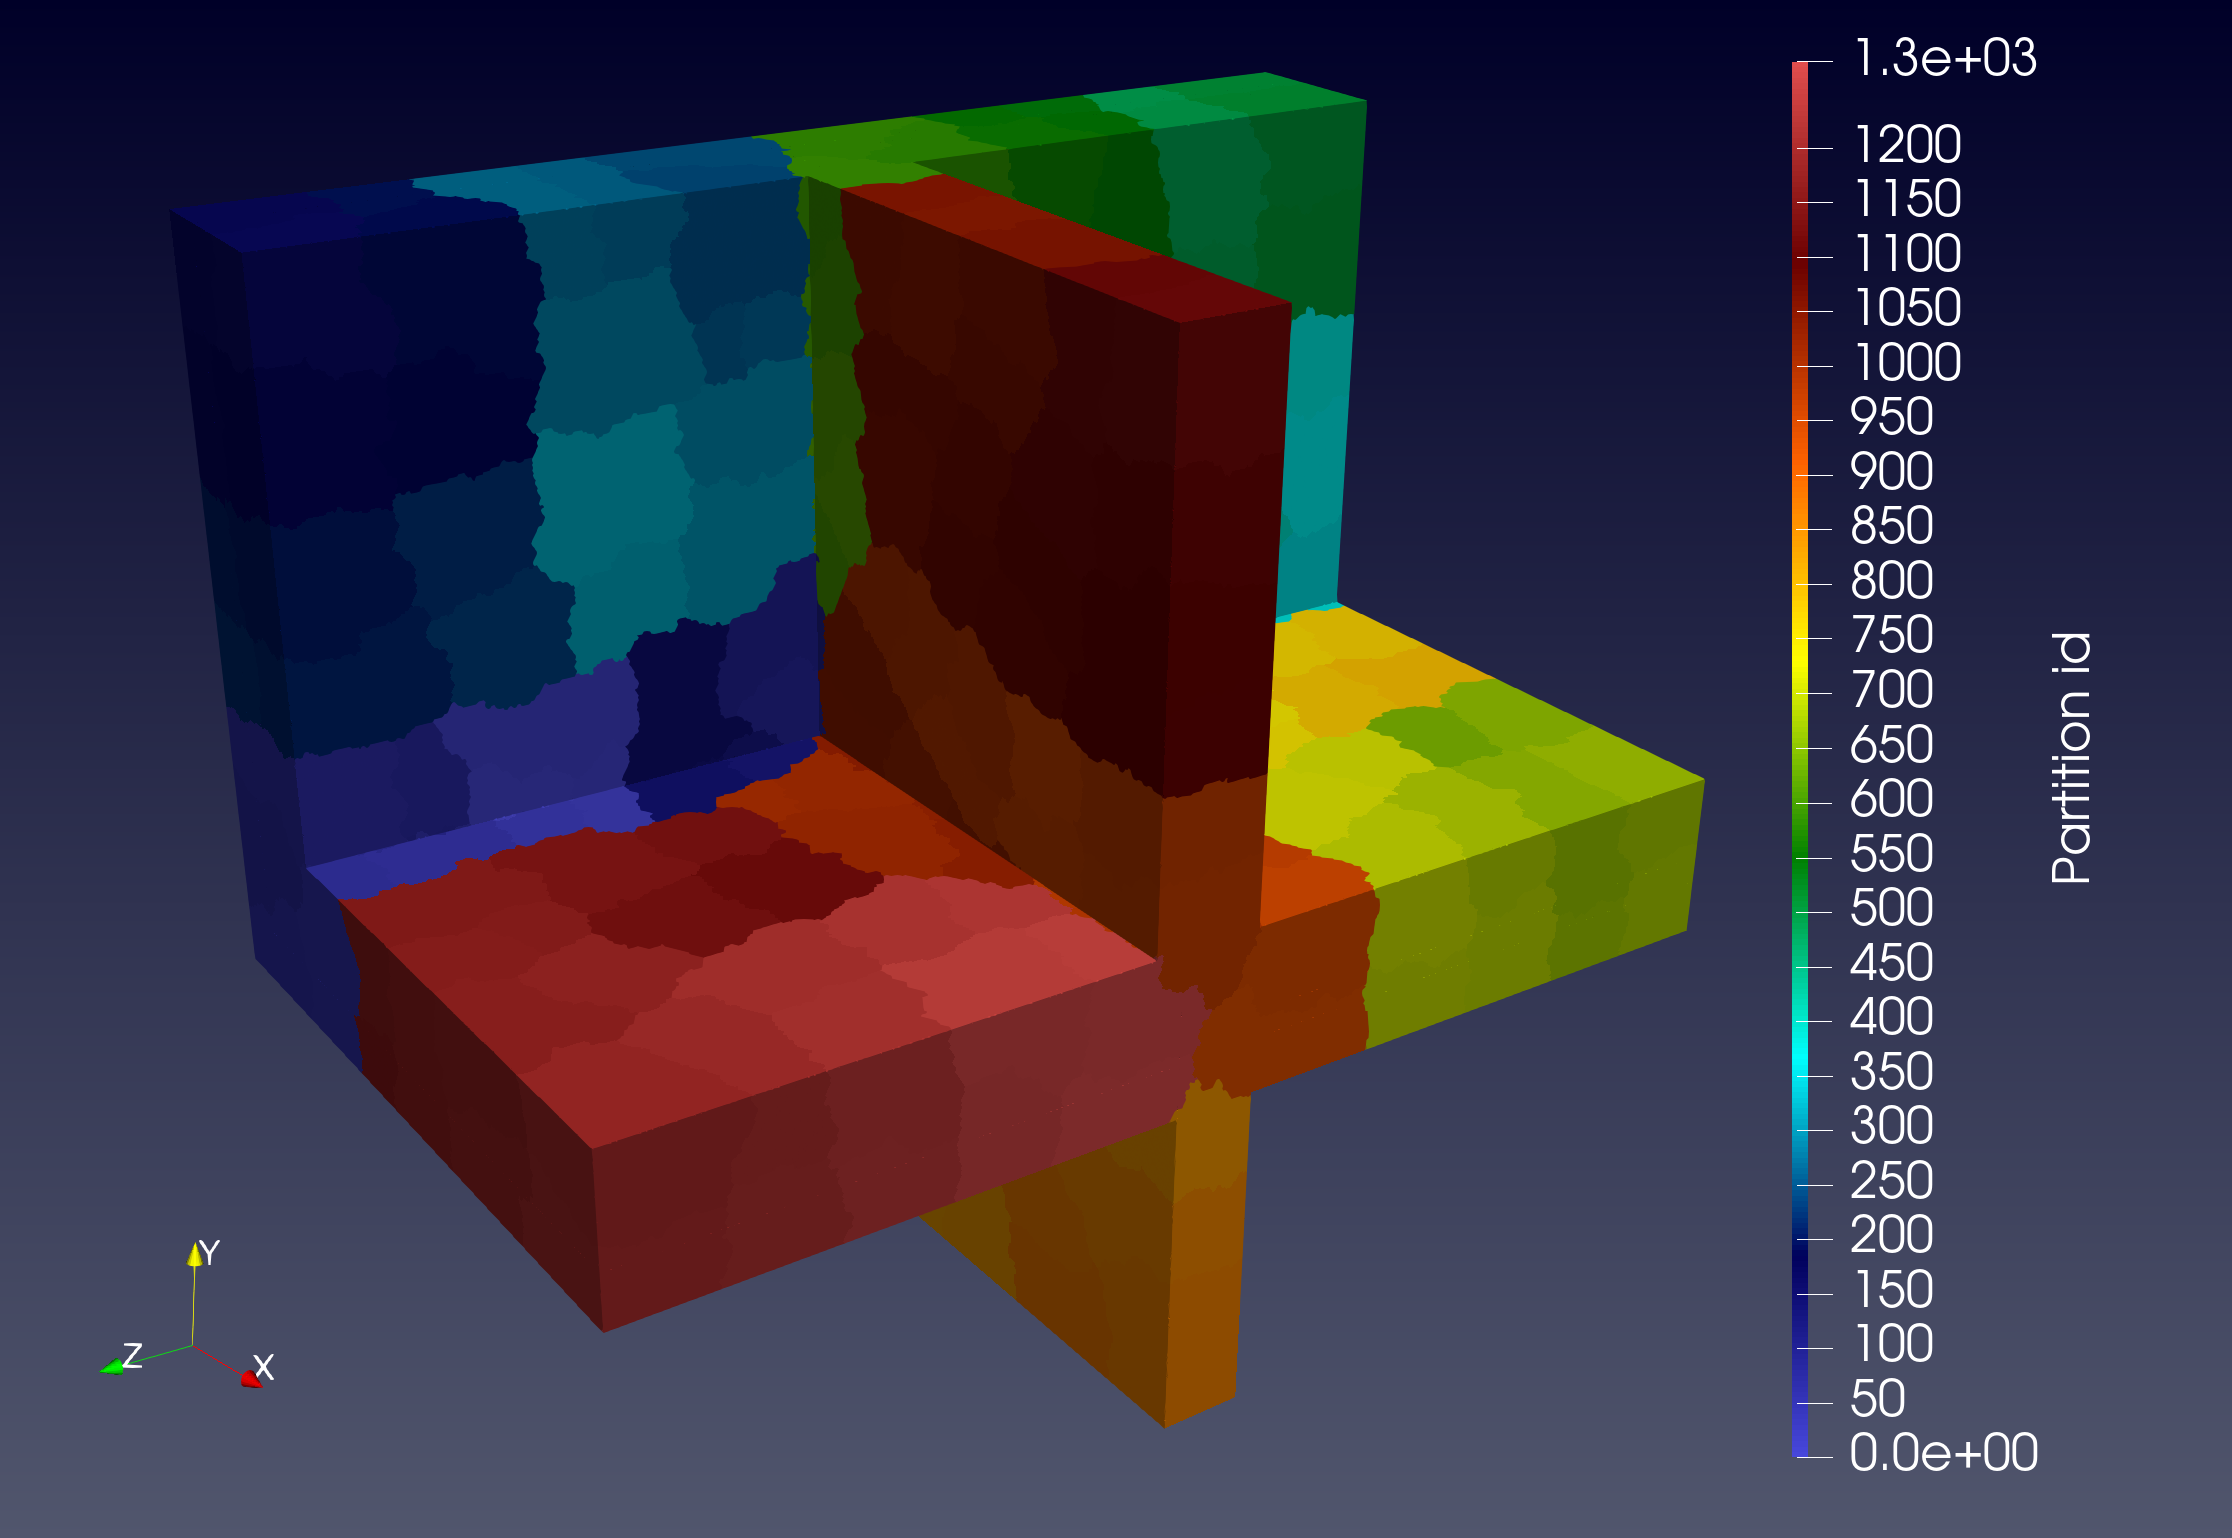
\includegraphics[width=\textwidth]{graphics/feelpp/feelpp-benchmark-thermalbridges-pid.png}
  \end{subfigure}
  \caption{Thermal bridges benchmarks - temperature solution (left) and
    partitioning example (right)}
  \label{fig:spec:app-feelpp-discr-1:thermal_bridges:visualization}
\end{figure}


\subsubsection{Mesh convergence}

The convergence study validates the numerical accuracy of the \Feelpp implementation against the reference values provided by the ISO 10211:2017 standard. \Cref{fig:spec:app-feelpp-discr-1:thermal_bridges:measures_convergences} presents the convergence of key validation measures as a function of mesh refinement level.

The results demonstrate excellent agreement with reference values (shown as red dashed lines) for all three finite element orders ($\mathP_1$, $\mathP_2$, $\mathP_3$). Key observations include:
\begin{itemize}
\item \textbf{Heat flux measurements:} All three polynomial orders converge to the reference values for heat flow measurements in the $\alpha$, $\beta$, and $\gamma$ environments (46.09 W, 13.89 W, and 59.98 W respectively).
\item \textbf{Temperature measurements:} The minimum surface temperature in the $\alpha$ environment converges to the reference value of 11.32°C across all mesh levels.
\item \textbf{Convergence rates:} Higher-order finite elements ($\mathP_2$ and $\mathP_3$) achieve better accuracy on coarser meshes, demonstrating the efficiency of high-order methods for smooth solutions.
\item \textbf{Tolerance compliance:} All computed values fall within the tolerances specified by the ISO standard, confirming the correctness of the implementation.
\end{itemize}

The benchmark metric \texttt{benchmark-verification} confirms that the \Feelpp thermal toolbox meets the accuracy requirements for building thermal analysis applications.


\begin{figure}[ht]
  \centering
  \captionsetup[subfigure]{justification=centering}

  \pgfplotstableread[col sep=comma]{chapters/applications/specs/data/app-feelpp-discr-1/thermalbridges_measures.csv}\dataTableMeasures
  \def\myLineWidth{2pt}
  \def\myLineStyleA{loosely dashdotdotted}
  \def\myLineStyleB{dashed}
  \def\myLineStyleC{solid}

  \def\myAddPlot#1#2#3#4{
    \addplot[#3,every mark/.append style={solid},
      x filter/.code={
        \pgfmathparse{\thisrow{PolyOrder}==#2}
        \ifnum0=\pgfmathresult
        \pgfmathsetmacro{\newx}{nan}
      \else
        \pgfmathsetmacro{\newx}{\thisrow{Mesh}}
      \fi
      \pgfmathparse{\newx}
      },
      y filter/.expression={ #4*\pgfmathresult }
    ] table [x=Mesh, y=#1] {\dataTableMeasures};
  }

  \def\myPlotOutputMeasures#1#2#3#4{
    \resizebox{\textwidth}{0.6172\textwidth}{
      \begin{tikzpicture}
        \begin{axis}[
          width=\textwidth, height=0.6172\textwidth,
          xtick=data,
          xticklabel={M$\pgfmathprintnumber{\tick}$},
          xmajorgrids=true,
          ymajorgrids=true, yminorgrids=true,
          minor y tick num=2,
          xlabel={Mesh levels}, ylabel={#4},
          legend style={at={(0.,1)}, anchor=south west,font=\small,legend columns=4},
          ]

          \myAddPlot{#1}{1}{color=customdarkblue,\myLineStyleC,mark=o,line width=\myLineWidth}{#2}
          \addlegendentry{P1}
          \myAddPlot{#1}{2}{color=customcyan,\myLineStyleC,mark=triangle,line width=\myLineWidth}{#2}
          \addlegendentry{P2}
          \myAddPlot{#1}{3}{color=customorange,\myLineStyleC,mark=square,line width=\myLineWidth}{#2}
          \addlegendentry{P3}
          \addplot+[color=red,\myLineStyleB,mark=none,line width=\myLineWidth,every mark/.append style={solid}] coordinates {
            (1,#3) (3,#3)
          };
          \addlegendentry{Ref}

        \end{axis}
      \end{tikzpicture}
    }

  }

  \begin{subfigure}[c]{0.49\textwidth}
    \centering
    \myPlotOutputMeasures{Normal_Heat_Flux_alpha}{1}{46.09}{Heat flow [W]}
    \caption{Heat flow measured in $\alpha$ environment}
  \end{subfigure}
  \hfill
  \begin{subfigure}[c]{0.49\textwidth}
    \centering
    \myPlotOutputMeasures{Normal_Heat_Flux_beta}{1}{13.89}{Heat flow [W]}
    \caption{Heat flow measured in $\beta$ environment}
  \end{subfigure}
  \hfill
  \begin{subfigure}[c]{0.49\textwidth}
    \centering
    \vspace*{0.03\textheight}
    \myPlotOutputMeasures{Normal_Heat_Flux_gamma}{-1}{59.98}{Heat flow [W]} % warning inverse
    \caption{Heat flow measured in $\gamma$ environment}
  \end{subfigure}
  \hfill
  \begin{subfigure}[c]{0.49\textwidth}
    \centering
    \vspace*{0.03\textheight}
    \myPlotOutputMeasures{Statistics_temperature_alpha_min}{1}{11.32}{Temperature
      [°C]}
    \caption{Surface temperature min in $\alpha$ environment}
  \end{subfigure}

  \caption{Thermal bridges benchmarks - Convergence of validation measures compared to references values}
  \label{fig:spec:app-feelpp-discr-1:thermal_bridges:measures_convergences}
\end{figure}



\subsubsection{Times of execution}

The performance analysis focuses on the scalability of the main computational components: initialization, assembly, solving, and post-processing. Execution times were measured on the Gaya supercomputer at Unistra for strong scalability tests, where the problem size remains constant while increasing the number of processors.

\Cref{fig:spec:app-feelpp-discr-1:thermal_bridges:performance_times_M1,fig:spec:app-feelpp-discr-1:thermal_bridges:performance_times_M2,fig:spec:app-feelpp-discr-1:thermal_bridges:performance_times_M3} present both grouped and stacked bar charts showing the execution time breakdown for each mesh level and polynomial order.
Due to large memory requirements, the M3 mesh was only tested with polynomial orders $\mathP_1$ and $\mathP_2$ for the Gaya cluster.

Key performance insights include:

\begin{itemize}
\item \textbf{Preprocessing:} The mesh loading and toolbox initialization (blue bars) shows good scalability, with decreasing times as processor count increases. This validates the efficiency of the parallel mesh partitioning strategy.

\item \textbf{Assembly:} The finite element assembly phase (purple bars) represents a significant portion of total time and scales well for all mesh levels. Higher-order elements ($\mathP_3$) require more assembly time due to increased quadrature points and local matrix sizes.

\item \textbf{Solve:} The linear system solve phase (cyan bars) exhibits a clear scaling limit of 1 node (128 cores).
    The M1 mesh appears to be too small to effectively showcase parallel efficiency, while M2 and M3 demonstrate better scalability due to larger problem sizes.
    However, the M2 and M3 meshes show a scaling limit of 1 node. Beyond this point, increasing the number of processes provides little or no additional performance benefit, and the solve time may increase.
   The use of preconditioned GMRES contributes to efficient convergence, but communication overhead becomes more pronounced at higher processor counts.

\item \textbf{Post-processing:} The export and validation phase (orange bars) remains relatively constant across processor counts, as it involves I/O operations that are less amenable to parallelization.

\item \textbf{Strong scalability:} The total execution time decreases as the number of processors increases, demonstrating effective parallel efficiency. The speedup is particularly pronounced for the larger meshes (M2 and M3) where the computational workload per processor remains substantial.

\item \textbf{Load balancing:} The consistent performance across different processor counts indicates effective domain decomposition and minimal load imbalance.
\end{itemize}

The benchmark metric \texttt{strong-scalability} highlights the parallel performance of the current \Feelpp implementation and identifies a scaling limit at 128 cores for the solve phase.


\foreach [expand list=true] \meshId in {1,2,3} {

  \pgfplotstableread[col sep=comma]{chapters/applications/specs/data/app-feelpp-discr-1/thermalbridges_M\meshId_P1_gaya.csv}\dataPa
  \pgfplotstableread[col sep=comma]{chapters/applications/specs/data/app-feelpp-discr-1/thermalbridges_M\meshId_P2_gaya.csv}\dataPb

  \pgfplotstableread[col sep=comma]{chapters/applications/specs/data/app-feelpp-discr-1/thermalbridges_M\meshId_P1_speedup_gaya.csv}\dataSpeedupPa
  \pgfplotstableread[col sep=comma]{chapters/applications/specs/data/app-feelpp-discr-1/thermalbridges_M\meshId_P2_speedup_gaya.csv}\dataSpeedupPb

  \ifnum\meshId<3
    \pgfplotstableread[col sep=comma]{chapters/applications/specs/data/app-feelpp-discr-1/thermalbridges_M\meshId_P3_gaya.csv}\dataPc
    \pgfplotstableread[col sep=comma]{chapters/applications/specs/data/app-feelpp-discr-1/thermalbridges_M\meshId_P3_speedup_gaya.csv}\dataSpeedupPc
  \fi

  \begin{figure}
    \centering
    \def\plotSetup##1{
      {table=##1,column=Preprocessing,legend=Preprocessing,color=customdarkblue},
      {table=##1,legend=Assembly,column={Algebraic assembly},color=custompurple},
      {table=##1,legend=Solve,column={Algebraic solve},color=customcyan},
      {table=##1,legend=PostProcess,column=Postprocess,color=customorange}
    }
    \def\chartBarPlot##1##2{
      \barChart[ybar,
      width=\textwidth, height=0.6172\textwidth,
      xticklabels from table={##2}{resources.tasks},
      legend style={at={(0.5,1)}, anchor=south,font=\tiny,legend columns=-1}
      ]{\plotSetup{##1}}
    }

    \def\speedupPlot##1##2{
      \begin{tikzpicture}
        \begin{axis}[
          width=0.97\textwidth, height=0.6172\textwidth,
          ymin=0,
          xlabel={Tasks},
          ylabel={Speedup},
          xtick=data,
          xticklabels from table={##2}{resources.tasks},
          x tick label style={ rotate=-45 },
          xticklabel style={font=\small},
          yticklabel style={font=\small},
          ymajorgrids=true, grid style={dashed, gray!40},
          legend style={at={(0.5,1.02)}, anchor=south, font=\tiny, legend columns=3}
        ]
          % Plot optimal and half-optimal bounds
          \addplot[thick, dashed, color=black] table [x expr=\coordindex, y=optimal] {##2};
          \addlegendentry{Optimal}

          \addplot[thick, dotted, color=black] table [x expr=\coordindex, y=half-optimal] {##2};
          \addlegendentry{Half-optimal}

          % Plot actual speedup
          \addplot[thick, mark=*, mark size=1.5pt, color=customdarkblue] table [x expr=\coordindex, y=Preprocessing] {##2};
          \addlegendentry{Preprocessing}

          \addplot[thick, mark=square*, mark size=1.5pt, color=custompurple] table [x expr=\coordindex, y={Algebraic assembly}] {##2};
          \addlegendentry{Assembly}

            \addplot[thick, mark=triangle*, mark size=1.5pt, color=customcyan] table [x expr=\coordindex, y={Algebraic solve}] {##2};
          \addlegendentry{Solve}

          \addplot[thick, mark=diamond*, mark size=1.5pt, color=customorange] table [x expr=\coordindex, y=Postprocess] {##2};
          \addlegendentry{PostProcess}
        \end{axis}
      \end{tikzpicture}
    }

    \begin{subfigure}[c]{0.49\textwidth}
      \centering
      \chartBarPlot{dataPa}{\dataPa}
      \caption{\texttt{M\meshId} - \texttt{$P_1$}}
    \end{subfigure}
    \hfill
    \begin{subfigure}[c]{0.49\textwidth}
      \centering
      \speedupPlot{dataSpeedupPa}{\dataSpeedupPa}
      \caption{\texttt{M\meshId} - \texttt{$P_1$}}
    \end{subfigure}
    \hfill
    \vspace*{0.04\textwidth}
    \begin{subfigure}[c]{0.49\textwidth}
      \centering
      \chartBarPlot{dataPb}{\dataPb}
      \caption{\texttt{M\meshId} - \texttt{$P_2$}}
    \end{subfigure}
    \hfill
    \begin{subfigure}[c]{0.49\textwidth}
      \centering
      \speedupPlot{dataSpeedupPb}{\dataSpeedupPb}
      \caption{\texttt{M\meshId} - \texttt{$P_2$}}
    \end{subfigure}
    \ifnum\meshId<3
        \hfill
        \vspace*{0.04\textwidth}
        \begin{subfigure}[c]{0.49\textwidth}
          \centering
          \chartBarPlot{dataPc}{\dataPc}
          \caption{\texttt{M\meshId} - \texttt{$P_3$}}
        \end{subfigure}
        \hfill
        \begin{subfigure}[c]{0.49\textwidth}
          \centering
          \speedupPlot{dataSpeedupPc}{\dataSpeedupPc}
          \caption{\texttt{M\meshId} - \texttt{$P_3$}}
        \end{subfigure}
        \caption{Thermal bridges benchmarks - Execution time of main simulation components
          - Mesh \texttt{M\meshId} - Gaya}
    \fi
    \label{fig:spec:app-feelpp-discr-1:thermal_bridges:performance_times_M\meshId}
  \end{figure}
}

\subsubsection{Scalability on I/O}

The I/O scalability analysis examines the performance of mesh loading and solution export operations as the number of processors and mesh size vary. The benchmark metric \texttt{io-scaling} measures the time required for file system operations during initialization and post-processing phases.

Key I/O performance characteristics observed:
\begin{itemize}
\item \textbf{Parallel mesh loading:} The pre-partitioned mesh format (JSON+HDF5) enables efficient parallel loading, with read times scaling inversely with processor count. The initialization times shown in the performance charts demonstrate this scalability.

\item \textbf{Export operations:} Writing visualization files (EnSight Gold format) exhibits limited scalability due to file system contention when multiple processors write simultaneously. This is evident in the relatively constant post-processing times across different processor counts.

\item \textbf{Mesh size impact:} Larger meshes (M3 with 10.5M vertices) show more pronounced I/O bottlenecks compared to smaller meshes (M1 with 193K vertices), as the absolute amount of data written increases significantly.

\item \textbf{Recommendations:} For production runs, using collective I/O strategies and reducing the frequency of visualization exports can significantly improve overall performance. The HDF5-based mesh format provides good parallel I/O performance for mesh loading operations.
\end{itemize}

These I/O characteristics are typical for large-scale finite element simulations and inform best practices for configuring output frequencies in production simulations.
